

\section{Implementation}
Most of the theorie behind RS and the methodology it depends on have already been introduced.
The implementation of a RS will be described in the following.
The examples will be written in a programming language called Python.
There is also some SQL code and some UML- and EER-diagrams in order to visualize the concept.

\subsection{Content based RS in-depth}
\label{sec:implementation-contentbased}
The general framework for a content-based RS is shown in figure~\ref{fig:framework-contentbasedrs}.
There are three main components a content-based RS needs.
\begin{itemize}
    \item \textbf{Content Analyzer}\\
        Since all items the RS has to work with can potentially be unstructured, a pre-process is necessary to filter relevant information.
        This will be mainly done by techniques of IR.
        The Content Analyzer aims to bring all items in a from that can be used by its successional components.
        \citep[p.~75-77]{lops:2011}
    \item \textbf{Profile Learner}\\
        When the items are in a suitable form, the Profile Learner can construct a user profile.
        In case of Rocchio's algorithm this includes to distinguish all relevant items from non-relevant.
        With the items and the users preferences the Profile Learner can build the user profile.
        In case of Rocchio, the user profile is a vector representing his attitude towards the different attributes a item may have.
        \citep[p.~75-77]{lops:2011}
    \item \textbf{Filtering Component}\\
        For each user profile the Filtering Component can find items that may match the users preferences.
        Depending on the method implemented the result can be a binary or continuous relevance judgment.
        The continuous relevance judgement is a list of ranked items.
        \citep[p.~75-77]{lops:2011}
        The RS implemented for this thesis uses the k-nearest-neighbours (kNN) classification.
        This results in a list of ranked items where the $k$ best-ranked items will be suggested to the user.
\end{itemize}


\begin{figure}[h]
    \center
    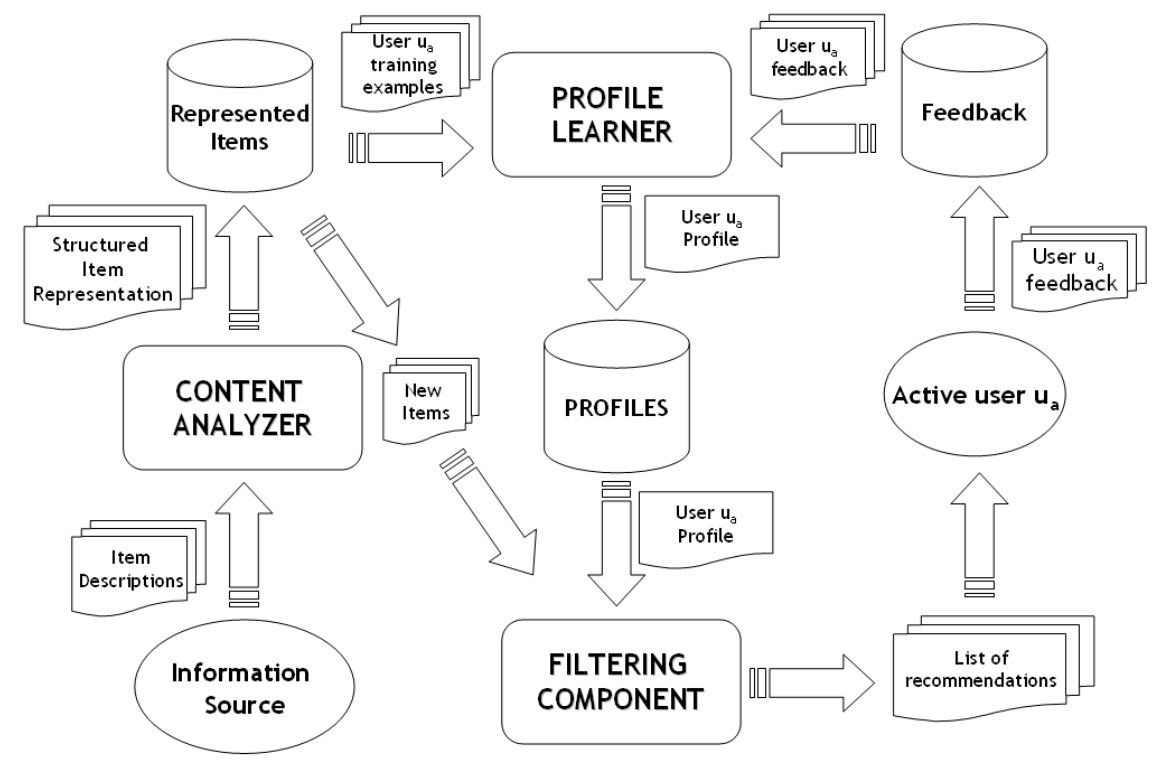
\includegraphics[scale=0.3]{inc/implementation/HighlevelContentBased}
    \caption{High level description of a content-based RS.\citep[p.~76]{lops:2011}}
    \label{fig:framework-contentbasedrs}
\end{figure}

\subsection{Content Analyzer}
%{Building the vectors}
%{Storage within the database}
For this project the data describing the products, offered by an online shop have been semi-structured.
It was a text file where each line described a product.
An example is given im figure~\ref{fig:productdata}.
\begin{figure}[h]
\begin{lstlisting}
ImgURL Brand Product Price Shoulder_Width Model_Length Collar_Type Material
http://i1.ztat.net/large/4E/M2/1E/00/0K/11/4EM21E000-K11@4.jpg Emoi en Plus Bluse - dazzling blue 24,95 °(\euro{})° 50 cm 70 cm bei Gr°(\"{o}\ss{})°e 44 Rundhals 100% Polyester
http://i2.ztat.net/large/NA/52/1D/03/NA/11/NA521D03N-A11@3.jpg NAF NAF WENT - Bluse - ecru/noir 38,95 °(\euro{})° 55 cm bei Gr°(\"o{}\ss{})°e S Rundhals 64% Viskose, 22% Baumwolle, 10% Modal, 4% Polyamid
\end{lstlisting}
    \caption{Example product data}
    \label{fig:productdata}
\end{figure}
Since the structure of the input was known, it was possible to filter out all relevant product information without using too fancy IR methods.
With regular expressions all relevant informations such as the product\_image-url, brand, product, price, collar type and material have been extracted and stored in a database.
Since a RS could theoretically handle any kind of item afar from products, a distinction has been made between documents in general and products.
The relation between a product and a document has been illustrated in figure~\ref{fig:ertermdocumentassignment}.
It is notable that all terms in a document are treated equally.
This means, that there are no parametric zones or such (section~\ref{sec:parametricandzoneindices}).
\begin{figure}[h]
    \center
    \includegraphics[scale=0.5]{inc/implementation/er_term_document_assignment}
    \caption{ER diagram of documents, products and associated terms}
    \label{fig:ertermdocumentassignment}
\end{figure}
Since the relation between \textit{Product} and \textit{Term} is N to N, an intermediate table is neccessary when transforming the ER-diagram into a relational model.
Therefore the table \textit{TermDocumentAssigner} will be introduced and the relational model will look as follows:

\begin{quote}
    \textbf{Document}{(\underline{document\_id})}\\
    \textbf{Product}{(\underline{document\_id[Document]}, image\_name)}\\
    \textbf{Term}{(\underline{term\_id}, name)}\\
    \textbf{TermDocumentAssigner}{(\underline{document\_id[Document], term\_id[Term]}, count)}\\
\end{quote}
\noindent
Since \textit{TermDocumentAssigner} will be very often used to query all terms of a document, it is useful to make an index on \textit{document\_id}.
Implicitly there will also be one on the combined primary key \textit{document\_id, term\_id}.
The tables, implemented by the RS build for this thesis, filled with example data may look as in table~\ref{tab:tablestermdocumentproduct}.
Table~\ref{tab:tablestermdocumentproduct} will serve as resource for terms and documents to illustrate subsequent examples.\\

\begin{table}

    \center

    % Document
    \rowcolors{1}{\dustRowFirst}{\dustRowSecond}
    \begin{tabular}{ l }
        \rowcolor{\dustRowHead}
        \textbf{Document}\\\hline
        document\_id\\\hline
        1\\
        2\\
        3\\
    \end{tabular}
    \quad
    % Product
    \rowcolors{1}{\dustRowFirst}{\dustRowSecond}
    \begin{tabular}{ l | l }
        \rowcolor{\dustRowHead}
        \multicolumn{2}{ c }{\textbf{Product}}\\\hline
        document\_id    & image\_name\\\hline
        1               & image\_1.png\\
        2               & image\_2.png\\
        3               & image\_3.png\\
    \end{tabular}

    ~\\

    %TermDocumentAssigner
    \rowcolors{1}{\dustRowFirst}{\dustRowSecond}
    \begin{tabular}{ l | l | l }
        \rowcolor{\dustRowHead}
        \multicolumn{3}{c}{\textbf{TermDocumentAssigner}}\\\hline
        document\_id    & term\_id  & count\\\hline
        1               & 1         & 1\\
        1               & 2         & 1\\
        1               & 4         & 1\\
        2               & 1         & 1\\
        2               & 3         & 1\\
        2               & 7         & 1\\
        3               & 4         & 1\\
        3               & 5         & 1\\
        3               & 6         & 1\\
    \end{tabular}
    \quad
    % Term
    \begin{tabular}{ l | l }
        \rowcolor{LightSlateGrey}
        \multicolumn{2}{ c }{\textbf{Term}}\\\hline
        term\_id        & name\\\hline
        1               & blouse\\
        2               & blue\\
        3               & polyester\\
        4               & cotton\\
        5               & green\\
        6               & trouser\\
        7               & white\\
    \end{tabular}
    \caption{Table layout defined by figure~\ref{fig:ertermdocumentassignment}}
    \label{tab:tablestermdocumentproduct}
\end{table}

\noindent
As already mentioned before, Rocchio's algorithm works best with tf-idf vectors.
Since the theory has been described in section~\ref{sec:tfidf}, the next big step is to show how vectors for this project have been built.
A short reminder: currently all products are described through their terms.\\

In order to build tf-idf vectors, one also has to built term frequency, as well as inverse document frequency vectors - these are the preconditions.
Since these tasks are fairly similar, some design patterns help realizing them.
The abstract factory pattern (described in section~\ref{sec:abstractfactory}) proofed to be very handy for this task.
For each necessary vector (tf, idf, tf-idf) one can build a vector creator which shares the design of the other vector creators.
Therefore the abstract class \textit{VectorCreator} has been introduced.
The \textit{VectorCreator} offers the abstract method \textit{\_get\_vector(document\_id:int):DocumentVector} which will be responsible for creating all vectors.
All inherited classes will implement the abstract method with a procedure to create an instance of \textit{DocumentVector}.

\paragraph{Term frequency vector}
Every term frequency vector representing a document consists of the term frequency of all terms.
The current implementation uses the SQL query displayed in figure~\ref{fig:tf-query} for generating the tf vector.
The result of a query may look as follows (based on the tables shown in figure~\ref{fig:ertermdocumentassignment} and are displayed in table~\ref{tab:tf-query-result}.
\begin{table}
    \begin{tabular}{ l|l|l || l|l|l || l|l|l }
        \rowcolor{LightSlateGrey}
        \multicolumn{3}{c||}{\textbf{$\text{tf}_\text{document\_1}$}} &
        \multicolumn{3}{c||}{\textbf{$\text{tf}_\text{document\_2}$}} &
        \multicolumn{3}{ c }{\textbf{$\text{tf}_\text{document\_3}$}}\\\hline
        
        term\_id & name & count                    & term\_id & name & count                    & term\_id & name & count\\\hline
        1   & blouse    & 1                              & 1    & blouse    & 1                 & 1 & blouse  & 0\\
        2   & blue      & 1                              & 2    & blue      & 0                 & 2 & blue  & 0\\
        3   & polyester & 0                              & 3    & polyester & 1                 & 3 & polyester  & 0\\
        4   & cotton    & 1                              & 4    & cotton    & 0                 & 4 & cotton  & 1\\
        5   & green     & 0                              & 5    & green     & 0                 & 5 & green  & 1\\
        6   & trouser   & 0                              & 6    & trouser   & 0                 & 6 & trouser  & 1\\
        7   & white     & 0                              & 7    & white     & 1                 & 7 & white  & 0\\
    \end{tabular}
    \caption{Possible result of the query in figure~\ref{fig:tf-query}}
    \label{tab:tf-query-result}
\end{table}

\begin{figure}[h]
    \lstset{language=SQL}
    \begin{lstlisting}
-- :document_id is a parameter given to the method
SELECT
    [t].[term_id]
    , [t].[name]
    , CASE WHEN  [a].[document_id] IS NULL
        THEN    0
        ELSE    [a].[count]
    END AS [value]
FROM
    [Term] AS [t]
    LEFT OUTER JOIN [TermDocumentAssigner] AS [a]
        ON  [t].[term_id] = [a].[term_id]
        AND [document_id] = :document_id
ORDER BY    [t].[term_id]
;
    \end{lstlisting}
    \caption{SQL query for generating tf-vectors}
    \label{fig:tf-query}
\end{figure}

\noindent
The result of the query shown in figure~\ref{fig:tf-query} will finally be stored in the \textit{TermFrequencyVector} class derived from \textit{DocumentVector} (see figure~\ref{fig:uml-document-vectors}).

\paragraph{Document frequency vector}
In contrast to the \textit{TermFrequencyVector} the \textit{DocumentFrequencyVector} does not resemble a single document, rather than the whole collection of documents.
Therefore the parameter \textit{document\_id} can be omitted.
But in order to sustain uniformity between all classes inheriting from \textit{VectorCreator} it will be carried along but set to a null value.
To make the source code more readable, the SQL code for querying the document-frequency values has been outsourced to a SQL-View as shown in figure~\ref{fig:df-view}.
This little tweak (that has no influence on speed) left the query for df-vectors as simple as shown in figure~\ref{fig:df-query}.
The result for the example is given in table~\ref{tab:df-query-result}.

\begin{figure}[h]
    \lstset{language=SQL}
    \begin{lstlisting}
CREATE VIEW IF NOT EXISTS [DocumentFrequency] AS
    SELECT
            [t].[term_id]
            , [t].[name]
            , CASE WHEN   [a].[count] IS NULL
                THEN        0
                ELSE        [a].[count]
            END AS [value]
    FROM
        [Term] as [t]
        LEFT OUTER JOIN
        (
            SELECT
                [term_id]
                , SUM([document_id]) AS [count]
            FROM
                [TermDocumentAssigner]
            GROUP BY
                [term_id]
        ) AS [a]
            ON [t].[term_id] = [a].[term_id]
    ORDER BY
        [t].[term_id]
;
    \end{lstlisting}
    \caption{SQL statement to create the \textit{DocumentFrequency}-view}
    \label{fig:df-view}
\end{figure}

\begin{figure}[h]
    \lstset{language=SQL}
    \begin{lstlisting}
SELECT
    [term_id]
    , [name]
    , [count]
FROM
    [DocumentFrequency]
;
    \end{lstlisting}
    \caption{SQL query for generating df-vectors}
    \label{fig:df-query}
\end{figure}

\begin{table}
    \center
    \begin{tabular}{ l | l | l } 
        \rowcolor{LightSlateGrey}
        \multicolumn{3}{ c }{\textbf{df}}\\\hline
        term\_id    & name      & count\\\hline
        1           & blouse    & 2\\
        2           & blue      & 1\\
        3           & polyester & 1\\
        4           & cotton    & 2\\
        5           & green     & 1\\
        6           & trouser   & 1\\
        7           & white     & 1\\
    \end{tabular}
    \caption{Possible results of the query in figure~\ref{fig:df-query}}
    \label{tab:df-query-result}
\end{table}

\begin{figure}[h]
    \center
    \includegraphics[scale=0.4]{inc/implementation/uml_document_vectors}
    \caption{Document vectors}
    \label{fig:uml-document-vectors}
\end{figure}

\paragraph{Inverse document frequency vector}
For building idf-vectors one can use df-vectors (and their source code) as basis.
The inverse document frequency is calculated by dividing the document frequency through the total count of documents in a collection.
Another SQL-View called N-view will provide the number of documents, while the code for creating idf-vectors get outsourced into its own view once more.
Since the SQL implementation of \textit{sqlite3} does not offer a logarithm-function, one has to defined his very own.
Fortunately the standard python library for connecting to sqlite3-databases supports the creation of functions as shown in figure~\ref{fig:idf-view}.


\begin{figure}
    \lstset{language=Python}
    \begin{lstlisting}
def _create_log_function(sqlite3_conn):
    sqlite3_conn.create_function('log10', 1, log_10)
    pass

def log_10(x):
    base = 10
    return math.log(x, base)
    \end{lstlisting}
    \lstset{language=SQL}
    \begin{lstlisting}
CREATE VIEW IF NOT EXISTS [InverseDocumentFrequency] AS
    SELECT
        [term_id]
        , [name]
        , log10
        (
            CAST ((SELECT [document_count] from [N]) AS REAL) / [df].[value]
        ) AS [value]
    FROM
        [DocumentFrequency] AS [df]
    ORDER BY
        [term_id]
;
    \end{lstlisting}
    \caption{SQL-statement to create the InverseDocumentFrequency-view}
    \label{fig:idf-view}
\end{figure}


\begin{figure}
    \lstset{language=SQL}
    \begin{lstlisting}
CREATE VIEW IF NOT EXISTS [N] AS
    SELECT
        (SELECT COUNT(*) FROM [Document]) AS [document_count]
        , (SELECT COUNT(*) FROM [Term]) AS [term_count]
;
    \end{lstlisting}
    \caption{SQL-statement to create the N-view}
    \label{fig:n-view}
\end{figure}


\begin{figure}
    \lstset{language=SQL}
    \begin{lstlisting}
SELECT
    [term_id]
    , [name]
    , [value]
FROM
    [InverseDocumentFrequency]
;
    \end{lstlisting}
    \caption{SQL-query for generating idf-vectors}
    \label{fig:idf-query}
\end{figure}


\begin{table}
    \center
    \rowcolors{1}{\dustRowFirst}{\dustRowSecond}
    \begin{tabular}{ l | l | l } 
        \rowcolor{\dustRowHead}
        \multicolumn{3}{ c }{\textbf{idf}}\\\hline
        term\_id    & name      & count\\\hline
        1           & blouse    & $\log_{10}(3/2) \approx 0.18$\\
        2           & blue      & $\log_{10}(3/1) \approx 0.48$\\
        3           & polyester & $\log_{10}(3/1) \approx 0.48$\\
        4           & cotton    & $\log_{10}(3/2) \approx 0.18$\\
        5           & green     & $\log_{10}(3/1) \approx 0.48$\\
        6           & trouser   & $\log_{10}(3/1) \approx 0.48$\\
        7           & white     & $\log_{10}(3/1) \approx 0.48$\\
    \end{tabular}
    \caption{Possible results of the query in figure~\ref{fig:idf-query}}
    \label{tab:idf-query-result}
\end{table}




\noindent
The whole vector creation process is also illustrated in figure~\ref{fig:uml-vectorssimple}.
\begin{figure}[h]
    \center
    \includegraphics[scale=0.33,angle=90]{inc/implementation/uml_vectors_simple}
    \caption{Abstract and concrete vector fabric}
    \label{fig:uml-vectorssimple}
\end{figure}


\subsection{Profile Learner}
%{Rocchio algorithm}
%{Relevance feedback}

\subsection{Filtering Component}


%%%%%%%%%%%%%%%%%%%%%%%%%%
%k nearest neighbours
% manning 297, 290 (euclidean distance)
%%%%%%%%%%%%%%%%%%%%%%%%%%

\subsection{Online shop}
... dunno

\subsection{Testing and findings}
wie sind die Empfehlungen des algorithmus








